%%% he main file. It contains definitions of basic parameters and includes all other parts.

%% Settings for single-side (simplex) printing
% Margins: left 40mm, right 25mm, top and bottom 25mm
% (but beware, LaTeX adds 1in implicitly)
%\documentclass[12pt,a4paper]{report}
%\setlength\textwidth{145mm}
%\setlength\textheight{247mm}
%\setlength\oddsidemargin{15mm}
%\setlength\evensidemargin{15mm}
%\setlength\topmargin{0mm}
%\setlength\headsep{0mm}
%\setlength\headheight{0mm}
% \openright makes the following text appear on a right-hand page
%\let\openright=\clearpage

%% Settings for two-sided (duplex) printing
% urcite tiskni oboustranne, jednostranny bakalarky jsou fuj.
\documentclass[12pt,a4paper,twoside,openright]{report}
%
% btw haha, tady si ruzny matfyzaci mysleli ze umej typografii lip nez
% profesionalove co se tim zabejvaji poslednich 300 let. Kdyby ti prislo ze
% stranky jsou tedka "divne rozjety do stran", tak to je dobre a kazdej tiskar
% to pochvali. Pak nekdy kdyztak vysvetlim proc to tak je.
%
%\setlength\textwidth{145mm}
%\setlength\textheight{247mm}
%\setlength\oddsidemargin{14.2mm}
%\setlength\evensidemargin{0mm}
%\setlength\topmargin{0mm}
%\setlength\headsep{0mm}
%\setlength\headheight{0mm}
\let\openright=\cleardoublepage

%% Prefer Latin Modern fonts
\usepackage{lmodern}

%% Further useful packages (included in most LaTeX distributions)
\usepackage{amsmath}        % extensions for typesetting of math
\usepackage{amsfonts}       % math fonts
\usepackage{amsthm}         % theorems, definitions, etc.
\usepackage{bbding}         % various symbols (squares, asterisks, scissors, ...)
\usepackage{bm}             % boldface symbols (\bm)
\usepackage{graphicx}       % embedding of pictures
\usepackage{fancyvrb}       % improved verbatim environment
\usepackage[numbers]{natbib} % citation style AUTHOR (YEAR), or AUTHOR [NUMBER]
\bibliographystyle{plainnat} % this must be moved here for natbib to work correctly
\usepackage[nottoc]{tocbibind} % makes sure that bibliography and the lists
			    % of figures/tables are included in the table
			    % of contents
\usepackage{dcolumn}        % improved alignment of table columns
\usepackage{booktabs}       % improved horizontal lines in tables
\usepackage{paralist}       % improved enumerate and itemize
\usepackage{multicol}
\usepackage[usenames]{xcolor}  % typesetting in color
\usepackage{url}

\usepackage[textsize=tiny]{todonotes} %visual todo!

\usepackage{xspace}         %for......xspace.
\usepackage{fancyvrb}

\usepackage{pgfplots}
\pgfplotsset{compat=1.8}
\usepgfplotslibrary{statistics}


%% Generate PDF/A-2u
\usepackage[a-2u]{pdfx}

\usepackage{cleveref}       %\cref yay!

%% Character encoding: usually latin2, cp1250 or utf8:
\usepackage[utf8]{inputenc}

%%% Basic information on the thesis

% Thesis title in English (exactly as in the formal assignment)
\def\ThesisTitle{Object detection for video surveillance}

% Author of the thesis
\def\ThesisAuthor{Marek Dobranský}

% Year when the thesis is submitted
\def\YearSubmitted{2019}

% Name of the department or institute, where the work was officially assigned
% (according to the Organizational Structure of MFF UK in English,
% or a full name of a department outside MFF)
\def\Department{Department of Software Engineering}

% Is it a department (katedra), or an institute (ústav)?
\def\DeptType{Department}

% Thesis supervisor: name, surname and titles
\def\Supervisor{TODO}

% Supervisor's department (again according to Organizational structure of MFF)
\def\SupervisorsDepartment{The Department of Software Engineering}

% Study program and specialization
\def\StudyProgramme{Computer Science}
\def\StudyBranch{Artificial inteligence}

% An optional dedication: you can thank whomever you wish (your supervisor,
% consultant, a person who lent the software, etc.)
\def\Dedication{%
TODO
}

% Abstract (recommended length around 80-200 words; this is not a copy of your thesis assignment!)
\def\Abstract{%
TODO
}

\def\AbstractSK{
TODO
}

% 3 to 5 keywords (recommended), each enclosed in curly braces
\def\Keywords{%
TODO
}

%% The hyperref package for clickable links in PDF and also for storing
%% metadata to PDF (including the table of contents).
%% Most settings are pre-set by the pdfx package.
\hypersetup{unicode}
\hypersetup{breaklinks=true}

% Definitions of macros (see description inside)
%%% This file contains definitions of various useful macros and environments %%%
%%% Please add more macros here instead of cluttering other files with them. %%%

%%% Minor tweaks of style

% These macros employ a little dirty trick to convince LaTeX to typeset
% chapter headings sanely, without lots of empty space above them.
% Feel free to ignore.
\makeatletter
\def\@makechapterhead#1{
  {\parindent \z@ \raggedright \normalfont
   \Huge\bfseries \thechapter. #1
   \par\nobreak
   \vskip 20\p@
}}
\def\@makeschapterhead#1{
  {\parindent \z@ \raggedright \normalfont
   \Huge\bfseries #1
   \par\nobreak
   \vskip 20\p@
}}
\makeatother

% This macro defines a chapter, which is not numbered, but is included
% in the table of contents.
\def\chapwithtoc#1{
\chapter*{#1}
\addcontentsline{toc}{chapter}{#1}
}

% Draw black "slugs" whenever a line overflows, so that we can spot it easily.
\overfullrule=1mm

%%% Macros for definitions, theorems, claims, examples, ... (requires amsthm package)

\theoremstyle{plain}
\newtheorem{thm}{Theorem}
\newtheorem{lemma}[thm]{Lemma}
\newtheorem{claim}[thm]{Claim}

\theoremstyle{plain}
\newtheorem{defn}{Definition}

\theoremstyle{remark}
\newtheorem*{cor}{Corollary}
\newtheorem*{rem}{Remark}
\newtheorem*{example}{Example}

%%% An environment for proofs

%%% FIXME %%% \newenvironment{proof}{
%%% FIXME %%%   \par\medskip\noindent
%%% FIXME %%%   \textit{Proof}.
%%% FIXME %%% }{
%%% FIXME %%% \newline
%%% FIXME %%% \rightline{$\square$}  % or \SquareCastShadowBottomRight from bbding package
%%% FIXME %%% }

%%% An environment for typesetting of program code and input/output
%%% of programs. (Requires the fancyvrb package -- fancy verbatim.)

\DefineVerbatimEnvironment{code}{Verbatim}{fontsize=\small, frame=single}

%%% The field of all real and natural numbers
\newcommand{\R}{\mathbb{R}}
\newcommand{\N}{\mathbb{N}}

%%% Useful operators for statistics and probability
\DeclareMathOperator{\pr}{\textsf{P}}
\DeclareMathOperator{\E}{\textsf{E}\,}
\DeclareMathOperator{\var}{\textrm{var}}
\DeclareMathOperator{\sd}{\textrm{sd}}

%%% Transposition of a vector/matrix
\newcommand{\T}[1]{#1^\top}

%%% Various math goodies
\newcommand{\goto}{\rightarrow}
\newcommand{\gotop}{\stackrel{P}{\longrightarrow}}
\newcommand{\maon}[1]{o(n^{#1})}
\newcommand{\abs}[1]{\left|{#1}\right|}
\newcommand{\dint}{\int_0^\tau\!\!\int_0^\tau}
\newcommand{\isqr}[1]{\frac{1}{\sqrt{#1}}}

%%% Various table goodies
\newcommand{\pulrad}[1]{\raisebox{1.5ex}[0pt]{#1}}
\newcommand{\mc}[1]{\multicolumn{1}{c}{#1}}

%%% ie eg
\newcommand{\eg}{e.\,g.~}  % "exempli grata", "priklad zadarmo" Pis misto "For example" pokud je ten priklad kratkej.
\newcommand{\ie}{i.\,e.~}  % "Ic est", "to jest", dobry jako pomyslny rovnitko ve vete. Napr: rovnitko \ie ty dve rovny carky

%%% simpler \paragraph

\newcommand\para[1]{{\normalfont\normalsize\bfseries #1}\xspace}


\newcommand{\x}{$\times$}



% Title page and various mandatory informational pages
\begin{document}
%%% Title page of the thesis and other mandatory pages

%%% Title page of the thesis

\pagestyle{empty}
\hypersetup{pageanchor=false}
\begin{center}

\centerline{\mbox{
\includegraphics[width=166mm]{./img/logo-en.pdf}}}

\vspace{-8mm}
\vfill

{\bf\Large MASTER THESIS}

\vfill

{\LARGE\ThesisAuthor}

\vspace{15mm}

{\LARGE\bfseries\ThesisTitle}

\vfill

\Department

\vfill

\begin{tabular}{rl}

Supervisor of the bachelor thesis: & \Supervisor \\
\noalign{\vspace{2mm}}
Study programme: & \StudyProgramme \\
\noalign{\vspace{2mm}}
Study branch: & \StudyBranch \\
\end{tabular}

\vfill

% Zde doplňte rok
Prague 2019\YearSubmitted

\end{center}

\newpage

%%% Here should be a bound sheet included -- a signed copy of the "bachelor
%%% thesis assignment". This assignment is NOT a part of the electronic
%%% version of the thesis. DO NOT SCAN.

%%% A page with a solemn declaration to the bachelor thesis

\openright
\hypersetup{pageanchor=true}
\pagestyle{plain}
\pagenumbering{roman}
\vglue 0pt plus 1fill

\noindent
I declare that I carried out this bachelor thesis independently, and only with the cited
sources, literature and other professional sources.

\medskip\noindent
I understand that my work relates to the rights and obligations under the Act No.~121/2000 Sb.,
the Copyright Act, as amended, in particular the fact that the Charles
University has the right to conclude a license agreement on the use of this
work as a school work pursuant to Section 60 subsection 1 of the Copyright Act.

\vspace{10mm}

\hbox{\hbox to 0.5\hsize{%
In Prague date 2019	% FIXME!
\hss}\hbox to 0.5\hsize{%
signature of the author
\hss}}

\vspace{20mm}
\newpage



%%% Dedication

\openright

\noindent
\Dedication

\newpage

\openright
\pagestyle{plain}
\pagenumbering{arabic}
\setcounter{page}{1}

%%% Mandatory information page of the thesis

\openright

\vbox to 0.5\vsize{
\setlength\parindent{0mm}
\setlength\parskip{5mm}

Title:
\ThesisTitle

Author:
\ThesisAuthor

\DeptType:
\Department

Supervisor:
\Supervisor, \SupervisorsDepartment

Abstract:
\Abstract

Keywords:
\Keywords
\vss}

\newpage

%%% A page with automatically generated table of contents of the bachelor thesis
\tableofcontents
%%% Each chapter is kept in a separate file
\chapter*{Introduction}
\addcontentsline{toc}{chapter}{Introduction}


\paragraph{Related work}


\paragraph{Approach}

\paragraph{Thesis structure}
\chapter{Experiments}
\label{chap:exp}

In this chapter, we provide details on the techniques used to gather the data presented in the previous chapter. We also present additional experimental results.


\section{SSD Training}
\citeauthor{bib:ssd} implemented SSD model\footnote{\url{https://github.com/weiliu89/caffe/tree/ssd}} from their research paper using the \textit{Caffe}\footnote{\url{http://caffe.berkeleyvision.org/}} deep learning framework. We decided against performing our experiments in this, by now outdated framework, and implemented our version in newer \textit{PyTorch}\footnote{\url{https://pytorch.org/}} framework (more detailed technical specification of used libraries is available in \cref{app:impl}).

We started by implementing a common framework for SSD detectors, that would support SSD models with many modifications. Although SSDTC inference is possible in the same framework, we had to create a separate environment for the training (more on SSDTC in \cref{sec:ssdtcImpl}). 

The main characteristics of our framework are the use of \textit{SGD} optimizer \cite{bib:sgd} and the loss function defined for SSD, also called MultiBox loss (\cref{sec:ssd}). Another essential element of the detection pipeline, used for inference, is the non-maximum suppression algorithm. The parametrization of these modules can be seen in \cref{tab:trainParams}. It is also worth mentioning that for the sake of consistency, all experimental models were trained for 401 epochs with a batch size of 32, using those default parameters.

\begin{table}
    \centering
    \begin{tabular}{c c|c c| c c}
        \multicolumn{2}{c|}{MultiBox loss} & \multicolumn{2}{c|}{SGD optimizer} & \multicolumn{2}{c}{NMS} \\
        \hline
        IoU threshold & 0.5 & learning rate &  \num{e-3} & IoU threshold & 0.5\\
        \hline
        \multirowcell{2}{positive/negative\\ sample ratio} & \multirowcell{2}{1:3} & \multirowcell{2}{momentum} & \multirowcell{2}{0.9} & \multirowcell{2}{confidence \\ threshold} & \multirowcell{2}{0.2} \\
        & & & & & \\
        \hline
        & & weight decay & \num{5e-4} & & \\
    \end{tabular}
    \caption{A selection of default values for most important parameters in our framework. We used these values for training and evaluation in all experiments. Note that the learning rate decreases during the training.}
    \label{tab:trainParams}
\end{table}


\section{Measurements}
To make our work comparable to other similar studies and future works, we explain methods used for both precision and performance measurements.

\subsection{Precision}
Rather than implementing a copy of the precision evaluation, our precision measurements were taken using an external tool. Using the external tool, independent on our implementation, allows us to easily compare our results with other works with little to no modifications. We used the implementation by \citet{bib:metricsgit} that mirrors the evaluation process of the PASCAL VOC Challenge. The test setup used default parameters, meaning that the interpolation of AP was calculated using all data points and the IoU threshold was set to 0.5. 

We present all the measurements taken on Surveillance dataset while performing multiple experiments described in this thesis in \cref{tab:ap}.


\begin{table}
    \centering
    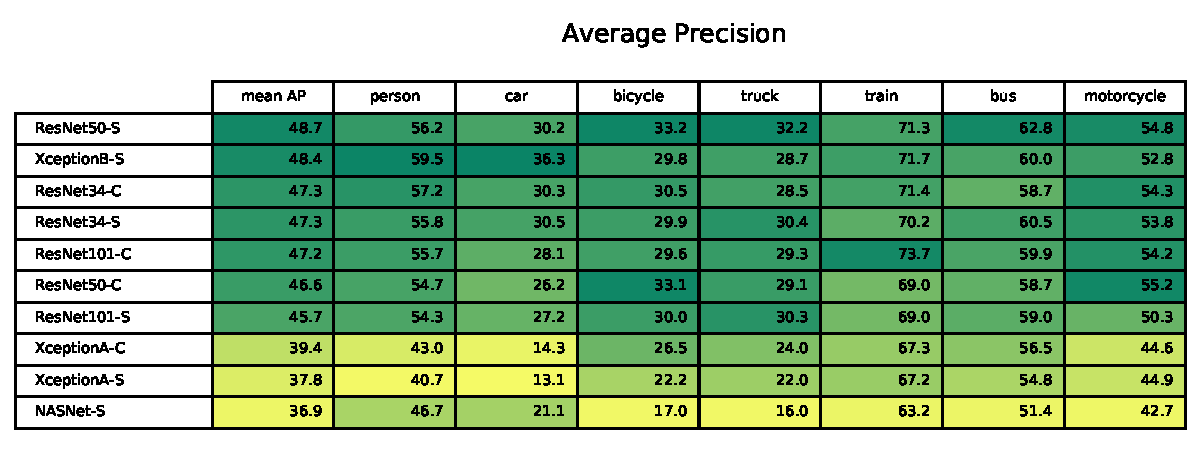
\includegraphics[width=\textwidth]{img/ap}
    \caption[Average precision of all tested networks on Surveillance classes]{Average precision of all tested networks on Surveillance classes. COCO indicates that the network was trained on COCO dataset, otherwise only Surveillance data were used for training.} 
    \label{tab:ap}
\end{table}

\subsection{Inference Speed}
The absolute values of the inference speed measurement would not provide any information without the knowledge of the environment in which they have been taken. In this section, we provide the details of both software and hardware environments used for measurements.

Testing was done by processing a total of 10 000 images in batches of 16. This process was timed, and the average \textit{fps} value was calculated.  Since we do not consider scaling and cropping the images to be part of the network, we did not need to include this process in the measurement. The set of [300\x300] pixel images was pre-loaded into memory before the timer was started. On the other hand, non-maximum suppression is a critical part of the algorithm and is included in the measurement. 

\paragraph{}
\noindent All our testing was done on the following hardware:
\begin{itemize}
    \item AMD EPYC 7401P CPU @ 2GHz \x 24
    \item NVIDIA GeForce GTX 1080 Ti
    \item 128GB DDR4 RAM
\end{itemize}


\section{Improving the Xception-SSD}
In \cref{sec:fixxception} we introduced a hypothesis about Xception\textit{A}-SSD. Based on this hypothesis, we presented the improved Xception\textit{H} model. However, as suggested by the name, it was not our first modification, and we needed some trial-and-error testing to achieve this result.

We will describe every iteration of the Xception-SSD model we trained and the reasoning behind the particular modifications. For clarity, we will refer to the Xception\textit{X} models in this section only by their version letters. The performance of mentioned models on Surveillance dataset is plotted on \cref{fig:xception_perf}, and more details on precision in \cref{tab:ap}. Also, the feature map sizes inside the models are shown in \cref{tab:xmods}.


\begin{figure}
    \centering
    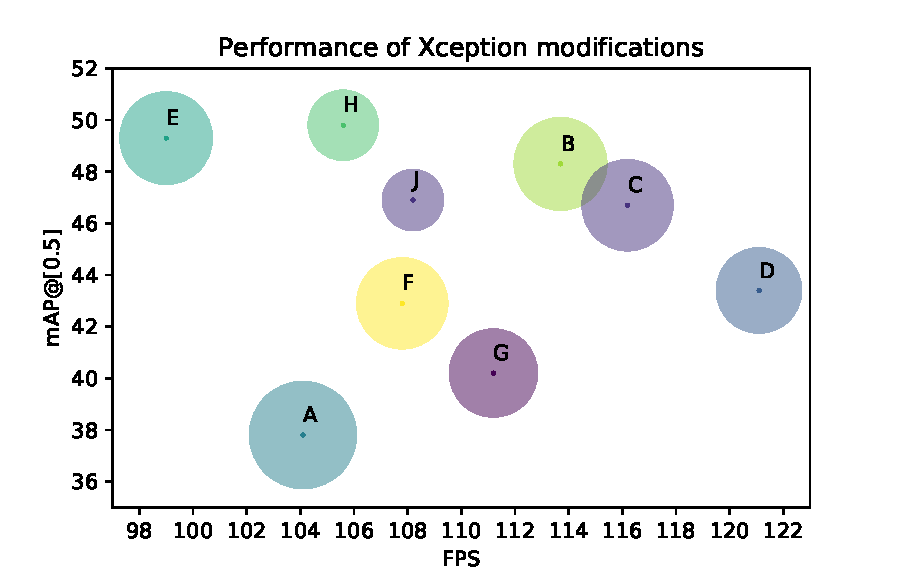
\includegraphics[width=0.95\textwidth]{img/fps_map_x}
    \caption[Performance of multiple Xception modification on Surveillance dataset]{Performance of multiple Xception modification on Surveillance dataset. Circle radii demonstrate relative difference of network parameter counts.} 
    \label{fig:xception_perf}
\end{figure}

\begin{table}
    \centering
    \begin{tabular}{c|c|c|c|c|c}
            &   A   &   B (C, D)   &   E (F, G)   &   H   &   J   \\
        \hline
        B1  &   [74\x128]   &   [74\x128]   &   [74\x128]   &   [74\x128]   &   [74\x128]   \\
        B2  &   \textbf{[37\x256]}   &  [37\x256]   &   [37\x256]   &   [37\x256]   &   [37\x256]   \\
        B3  &   [19\x728]   &   [19\x256]   &   [37\x256]   &   [37\x256]   &   [37\x256] \\
        \hline
        B4-6  &   [19\x728]   &   [19\x256]   &   [37\x256]   &   [37\x256]   &   [37\x256] \\
        B7  &   [19\x728]   &   \textbf{[19\x256]}   &   \textbf{[37\x256]}   &   \textbf{[37\x256]}   &   \textbf{[37\x256]} \\
        B8-10  &   [19\x728]   &   [19\x728]   &   [19\x728]   &   [19\x512]   &   [19\x512]\\
        B11 &   \textbf{[19\x728]}   &   \textbf{[19\x728]}   &   \textbf{[19\x728]}   &   \textbf{[19\x512]}   &   \textbf{[19\x512]}\\
        \hline
        B12 &   [10\x1024]  &   [10\x1024]  &   [10\x1024]  &   [10\x728]  &   [10\x512]\\
        S1  &   [10\x1536]  &   [10\x1536]  &   [10\x1536]  &   [10\x1024]  &   [10\x512]\\
        S2  &   \textbf{[10\x2048]}  &   \textbf{[10\x2048]}  &  \textbf{[10\x2048]}   &  \textbf{[10\x1024]} &  \textbf{[10\x512]}\\
    \end{tabular}
    \caption{A table of feature map sizes on the output of layers of the Xception networks. Bx stand for Xception blocks, S1 and S2 stand for separable convolution layers that follow the block structure (see \cref{fig:xception}). The first number represents spatial dimensions of a square feature, expecting [300\x300] input, and the second one represents the number of channels. The highlighted feature maps are used for the detections. The versions C, D, and F, G share the feature maps sizes with their parent versions, if the given layers are present, but do not match the highlighted feature extraction.}
    \label{tab:xmods}
\end{table}

\subsubsection{Versions B, C, D}
We examine this trio at once,  since version \textit{C} adds modifications to version \textit{B}, and version \textit{D} further modifies version \textit{C}. Notably, we trained these models in parallel and therefore had no results from concurrent models to inform on the design.

Starting with the assumption that the problem of the version \textit{A} is the position of the first feature extraction for detection, we moved the extraction from \textit{block 2} to \textit{block 7}. We also reduced the number of output filters on \textit{blocks 2 to 7} from 728 to 256. As a result, the first detection is performed on a [19\x19\x256] feature map as opposed to the [37\x37\x256] map of \textit{A}. The main factor here, it that the feature map is extracted after the data pass five additional blocks. 

Due to a reduction of feature map size, we considered this modification a half-measure in our plan to move the first feature extraction deeper into the network. However, it proved to be a successful step in the right direction. The network has significantly gained in both speed and precision values. 

Both versions \textit{C} and \textit{D} were designed for observation of the impact of the removal of parts of the network. We designed the modifications in such a way that they would not affect other layers. For clarity, the removals of blocks and layers do not alter the numbering scheme.

Version \textit{C} omits \textit{blocks 5, 6 and 7} and extracts the [19\x19] feature map after \textit{block 10} instead of \textit{block 11}. However, we did not observe a satisfying performance boost to justify received loss of precision. 

Version \textit{D} was designed to test the need for six detection layers, mainly the layers for detecting large objects. It is based on \textit{C} and removes the feature layers produced by \textit{extra layers}. Although the observed performance boost from \textit{C} to \textit{D} was more significant than the one from \textit{B} to \textit{C},  it was also coupled with a major precision penalty.

\subsubsection{Versions E, F, G}
Similarly to the previous trio, these versions are also based on each other, with the main architectural change being applied in \textit{E}. Versions \textit{F} and \textit{G} were designed to perform independent experiments. 

Version \textit{E} is the one, where we finally implemented our original intention of moving the first extracted feature map of [37\x37] size to a deeper layer. Implementation-wise, the only difference between \textit{B} and \textit{E}, is the removal of max-pooling with stride 2 from \textit{block 2} and placing it to \textit{block 8}. This movement results in the increase of feature size to the desired [37\x37] map up to \textit{block 8}.

We observed a noticeable drop-off in performance compared to version \textit{B} and a slight increase in precision. Although the number of parameters in the network is the same, the change from [19\x19] to [37\x37] requires about four times more computation per convolutional layer.

Version \textit{F} modifies \textit{E} in the same way, \textit{C} modified \textit{B}. It skips the \textit{blocks 5, 6 and 7} and extracts the second feature map after \textit{block 10}. Although the received performance boost in relation to \textit{E} is significant, the precision is also significantly impacted in a negative way.

Version \textit{G} repeated the experiment from version \textit{D}, but instead of removing the last three detection feature maps, we removed every other one, thus keeping the first, third and fifth ones. It is based on version \textit{F}, and again we see the precision loss we cannot justify by performance gain.

\subsubsection{Version H}
Since we managed to gain the best precision result with version \textit{E}, we decided to try and increase its performance. To this end, we designed the version \textit{H}. However, tests \textit{C}, \textit{F}, \textit{D} and \textit{G} showed that the removal of blocks or detection layers from the network is detrimental for the result. Therefore we decided for a less radical solution of trimming the channel depth of the network. We ended up trimming the [19\x19] feature map to 512 channels and [10\x10] map to 1024 channels.

Experiments show that this adjustment not only put the performance of the model halfway between \textit{E} and \textit{B} but also slightly boosted the precision.

\subsubsection{Version J}
After the success of version \textit{H}, we decided to try the limits of channel removal approach. We started with the setup of \textit{H}, and set the number of channels of every layer following \textit{block 7} up to \textit{extra layers}, to 512. 

Version \textit{J}, showed us, that this is also not a viable solution. The results are underwhelming in both, precision and performance.


\subsubsection{Conclusion}
In conclusion, we managed to receive the best precision results from the version \textit{H}. Our first implementation, \textit{A}, managed only 37.8\% mAP on Surveillance dataset. Meanwhile version \textit{H} achieved 49.8\% mA on the same data while keeping the performance equivalent.

\section{SSDTC Implementation and Training}
\label{sec:ssdtcImpl}
We have already described the architecture of SSDTC in \cref{sec:ssdtc}; however, the actual implementation and training process proved to be more complicated than SSD. In this section, we go through the challenges brought by SSDTC. 

As mentioned, we based the SSDTC on ResnNet34-SSD. We used the SSD initialized by the weights we learned on Surveillance dataset. We did not need the detection layers of SSD, so we removed them from the model. The resulting ResNet34 with \textit{extra layers} served as a feature extractor for both SSDTC and also for training the baseline SSD on HollywoodHeads dataset. For training of both networks, we froze the weights in the extractor and trained only temporal and detection layers. It is important to note that every image processed by SSDTC, passes through the same extractor. 

The SSDTC design we created, has different input data requirements for training and inference. To properly train, it needs a large number of smallest possible chunks in a batch for the network. However, one large chunk is the most effective way for inference and the most natural way as we expect a continuous video stream.

This, however, poses conflicting requirements for the implementation of the network, namely in the passing of data between the modules. For the purposes of explanation, lets call the ResNet34 network with \textit{extra} layers the \textit{Extractor}, the two conv3d layers the \textit{Temporal module}, and the localization and classification layers the \textit{Detection module}. We will also consider the detection process for only one of six feature map layers of the Extractor. 

During training, the network starts with feature extraction on seemingly independent \textit{n*c} frames in a batch (\textit{c} being the minimal possible chunk, in our case 5, and \textit{n} the batch size). Coming to the temporal layers, the feature maps need to be reshaped to represent \textit{n} chunks of size \textit{c} to allow for conv3d layers. After the temporal layers, the feature maps come out in the batch size of \textit{n}, but due to the nature of temporal layers, the chunk size is reduced to 1. This data then has to be reshaped again, to remove the temporal dimension, and create a batch of size \textit{n} for the detection layers.  

On the other hand, during inference, the input is a single chunk of consecutive frames, that is equivalent to a single batch. This batch can be simply passed thorough feature extraction layers, and the only modification needed for the temporal layers is to encapsulate the whole tensor in additional dimension to represent a temporal batch of size one. After the temporal convolution, we remove the encapsulation and continue with the detection; however, the batch size in this step is smaller than at the beginning. 

We can see the difference between training and inference feature sizes in \cref{tab:ssdtcFeatureSizes}. This behavior forced us into two separate implementations for inference and training. Although both implementations share the same network models, the differences are in the handling of the data between the modules. In the table, we can see that during training, it is the \textit{chunk dimension} that gets eliminated in temporal layers, and during the inference, it is the \textit{batch dimension}. 

Although it is possible to use both versions for training and inference, each has a significant disadvantage if not used as intended. The inference module does not allow for the use of the batch normalization in conv3d layers, because it operates with temporal volume in a batch size one. The fact that the ability to use batch normalization is vital for the training was also experimentally tested. Without normalization, we were not able to over-perform standard SSD with the temporal version. There is a better chance for the training module to be modified for efficient inference, although with some performance hit inherent from our implementation. 

\begin{table}
    \centering
    \begin{tabular}{c|c|c}
        Module &  \multicolumn{2}{c}{Training}\\
        \hline
            & Input   & Output    \\
        Extractor   &  [H$_0$\x W$_0$\x 3\x 5*N] & [H$_1$\x W$_1$\x F$_1$\x 5*N]  \\
        Temporal   &  [H$_1$\x W$_1$\x F$_1$\x 5\x N] & [H$_2$\x W$_2$\x F$_2$\x1\x N] \\
        Detector  &  [H$_2$\x W$_2$\x F$_2$\x N] &      \\
        \hline
        \multicolumn{1}{c}{} & \multicolumn{2}{c}{Inference}\\
         \hline
         & Input   & Output\\
        Extractor   &   [H$_0$\x W$_0$\x 3\x C]  & [H$_1$\x W$_1$\x F$_1$\x C]\\
        Temporal   &  [H$_1$\x W$_1$\x F$_1$\x C\x 1] & [H$_2$\x W$_2$\x F$_2$\x C-4\x 1]\\
        Detector   & [H$_2$\x W$_2$\x F$_2$\x C-4] & \\
        
    \end{tabular}
    \caption{Data shapes and sizes on the input and output of the SSDTC modules. The output of the Detector complies with SSD definitions (\cref{sec:ssd}).}
    \label{tab:ssdtcFeatureSizes}
\end{table}


\chapter{Artificial Neural Networks}
\label{chapt:nnets}
To better understand the the principles and limitation of object detection using artificial neural networks we will provide a brief overview of the basic concepts of artificial neural networks in this chapter. We will cover the principles behind single artificial neuron and algorithms used for training and inference on the network. Then we will focus on the composition of deep networks and their layers.

\section{Introduction to Artificial Neural Networks}
This section introduces the concept of artificial neuron and creating a network of them. We will take a deeper look at different functions and algorithms that make the network work and discuss the possible uses of such network.

\subsection{Artificial neuron}
\subsection{Activation Functions}
\subsection{Output Functions}
\subsection{Loss Functions}
\subsection{Back Propagation}
\subsection{Gradient Descent Optimization Algorithms}

\section{Layers of Neural Networks}
\subsection{Dense Layer}
\subsection{Convolutional Layer}
\subsection{Recurrent Cells}
\subsection{Normalization and Batch Normalization}

\section{Other useful Functions}
\subsection{Non-maximum Suppression}
\subsection{Hard Negative Mining}

\chapter{Convolutional Networks and Commonly Used Models}
\label{chapt:models}
\section{Precision Metrics}
mAP, IoU

\section{Commonly used datasets}
\label{datasets}
Pascal VOC, COCO, ImageNet, Open Image dataset

 vgg, resnet, ssd, fssd rfb

\section{Classification Networks}
\subsection{VGG}
\label{VGG}
\subsection{Inception}
\label{inception}
\subsection{ResNet}
\label{resnet}

All ResNet architectures (ResNet-10, ResNet-18, 34, 50...) use the same architecture (left chart), which is build from a few input layers, four sets of building blocks and output layers. Each of four blocks can be composed of multiple residual building blocks. There are two types of building blocks, larger block with three convolutional layers called "bottleneck", or smaller "basic" block with two convolutional layers.  see \cref{fig:resnet_arch}

\begin{figure}
    \label{fig:resnet_arch}

    \usetikzlibrary{shapes,arrows}
    
    
    % Define block styles

    \tikzstyle{block} = [rectangle, draw,  text centered, rounded corners, minimum height=2em]
    \tikzstyle{rect} = [rectangle, draw, text width=5em, text centered, minimum height=2em]
    \tikzstyle{head} = [rectangle, draw, fill=green!20, text width=9em, rounded corners, text centered, minimum height=2em]
    \tikzstyle{line} = [draw, -latex']
    \tikzstyle{cloud} = [draw, ellipse,fill=red!20, node distance=3cm,
        minimum height=2em]
    
    \begin{multicols}{3}   

        \subsection*{ResNet}
        \begin{tikzpicture}[every text node part/.style={align=center}, node distance=1.2cm]
            \node [block] (input) {Input};
            \node [block, below of=input] (conv1) {7x7 conv, 64, /2};
            \node [block, below of=conv1] (bn) {BatchNorm};
            \node [block, below of=bn] (relu) {ReLU};
            \node [block, below of=relu] (maxpool) {3x3 max pool, /2};
            \node [rect, below of=maxpool] (block1) {Block 1};
            \node [rect, below of=block1] (block2) {Block 2};
            \node [rect, below of=block2] (block3) {Block 3};
            \node [rect, below of=block3] (block4) {Block 4};
            \node [head, below of=block4] (avgpool) {Average Pooling};
            \node [head, below of=avgpool] (fc) {Fully connected (Classifier)};
            
            \path[line] (input) -- (conv1);
            \path[line] (conv1) -- (bn);
            \path[line] (bn) -- (relu);
            \path[line] (relu) -- (maxpool);
            \path[line] (maxpool) -- (block1);
            \path[line] (block1) -- (block2);
            \path[line] (block2) -- (block3);
            \path[line] (block3) -- (block4);
            \path[line] (block4) -- (avgpool);
            \path[line] (avgpool) -- (fc);
        
        \end{tikzpicture}
        \vfill\null
        \columnbreak
        
        \subsection*{Basic Block}
        \begin{tikzpicture}[every text node part/.style={align=center}, node distance=1.2cm]
            \node [block] (input) {Input};
            \node [block, below of=input] (conv1) {3x3 conv, 64*};
            \node [block, below of=conv1] (bn) {BatchNorm};
            
            \node [block, below of=bn] (relu) {ReLU};
            \node [block, below of=relu] (conv2) {3x3 conv, 64*};
            \node [block, below of=conv2] (bn2) {BatchNorm};
            \node  [block, below of=bn2] (plus) {+};
        
            \path[line] (input) -- (conv1);
            \path[line] (conv1) -- (bn);
            \path[line] (bn) -- (relu);
            \path[line] (relu) -- (conv2);
            \path[line] (conv2) -- (bn2);
             \path[line] (bn2) -- (plus);
            \path[line] (input) -| node [near end]{}([xshift=2.5cm] input.west)
                                |- (plus.east) coordinate (plus);
        
        \end{tikzpicture}
        \vfill\null
        \columnbreak
        
        \subsection*{Bottleneck Block}
        \begin{tikzpicture}[every text node part/.style={align=center}, node distance=1.2cm]
            \node [block] (input) {Input};
            \node [block, below of=input] (conv1) {1x1 conv, 64*};
            \node [block, below of=conv1] (bn) {BatchNorm};
            
            \node [block, below of=bn] (relu) {ReLU};
            \node [block, below of=relu] (conv2) {3x3 conv, 64*};
            \node [block, below of=conv2] (bn2) {BatchNorm};
            
            \node [block, below of=bn2] (relu2) {ReLU};
            \node [block, below of=relu2] (conv3) {1x1 conv, 256*};
            \node [block, below of=conv3] (bn3) {BatchNorm};
            
            \node  [block, below of=bn3] (plus) {+};
        
            \path[line] (input) -- (conv1);
            \path[line] (conv1) -- (bn);
            \path[line] (bn) -- (relu);
            \path[line] (relu) -- (conv2);
            \path[line] (conv2) -- (bn2);
            \path[line] (bn2) -- (relu2);
            \path[line] (relu2) -- (conv3);
            \path[line] (conv3) -- (bn3);
            \path[line] (bn3) -- (plus);
            \path[line] (input) -| node [near end]{}([xshift=2.5cm] input.west)
                                |- (plus.east) coordinate (plus);
        \end{tikzpicture}
    
    \end{multicols}
    
    \caption{Architecture of ResNet network.
    Note that the give number of convolutional filters is correct only for building blocks belonging to ResNets Block 1, otherwise the number doubles with each ResNet Block. Detailed specification can be found in }
\end{figure}
\todo{ref resnet documnet table 1}

maybe more

\section{Detection Networks}

\subsection{Region-based Convolutional Network (R-CNN)}
\subsubsection{R-CNN}
\subsubsection{Fast R-CNN}
\subsubsection{Faster R-CNN}

\subsection{You Only Look Once (YOLO)}
\subsubsection{YOLO}
\label{yolo}
\subsubsection{YOLO v2 and YOLO 9000}

\subsection{Single-Shot Detector (SSD)}
\label{ssd}
\subsubsection{SSD}

\subsubsection{FSSD}
\subsubsection{RFB}

\subsection{Mask Region-based Convolutional Network (Mask R-CNN)}

\section{Use of Detection networks for video processing}

%Optional section
\section{Other uses of CNNs}
\subsection{Noise removal/ Regularization}
\subsection{Image generation}




\chapter{Experiments}

\section{Experiments with Single-Shot Detector}
\label{chapt:experiments}
Based on our needs in terms of speed and accuracy we decided to base our first set of experiments on SSD detector (\cref{ssd}). The decision between SSD and YOLO (\cref{yolo}) was made by personal experience with SSD detector and it's application in real-time video analyses. However we decided replace the originally used VGG-16 network (\cref{VGG}) and instead build our detector atop the faster ResNet classifier (\cref{resnet}). We started our experiments with small ResNet-18, but the block structure of ResNet allows for using the same implementation of SSD-ResNet on any standard ResNet size, by using outputs of individual blocks as detectors inputs.

This section will describe the process of creating our SSD-ResNet network and multiple experiments performed in the course of development. We experimented with different methods of training the network, speed of inference based on the multiple parameters, we also tried training on artificial data for real-life applications.


\subsection{Building SSD on ResNet}
The task of building full SSD detector can be a little overwhelming without prior experience of building similar networks, so we decided to start with ResNet classifier and add localization layer. After successful implementation we went on to implement full detector. 

In order to verify the functionality and precision of our implementation we started by designing and implementing a simple artificial data generator. We chose to avoid using any common datasets (see \cref{datasets}) because of non-trivial preprocessing requirements. The detector will be trained on real data after it's functionality and viability are proven.

\subsubsection{Testing data}
We will be testing our implementation on artificial data generated on demand. We implemented simple generator for geometric shapes. We used squares, triangles and circles with fully randomized position, size, color and thickness. The triangles are in general position only conditioned by minimal ratio of circumference to area.
To make dataset harder, shapes are drawn over random background composed of the segments of the same shapes. The background shapes are never fully in the picture background. The example image seen be seen in \todo{example data}.



% resnet
% bla bla 10,18,32,50,101...

% feature map sized
% block1: 56x56
% block2: 28x28
% block3: 14x14
% block4: 7x7

% unlike original SSD on VGG-16 we decided to start with this basic setup without adding more feature layers, because we are interested in small objects on surveillance video and not for recognizing large objects on photographs.

% \begin{figure}
%     \centering
%     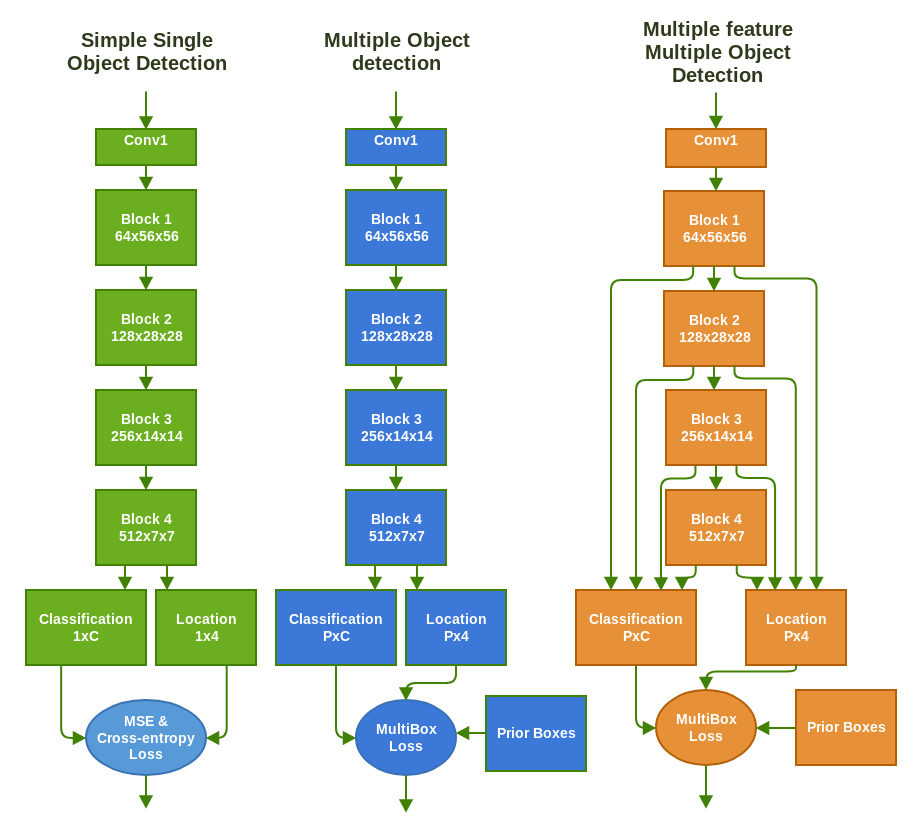
\includegraphics[width=\textwidth]{img/resnets.png}
%     \caption{High level structure of resnet with SSD}
%     \label{fig:resnet}
% \end{figure}





\subsubsection{Simple detector for one object}

optimizer = Adam(lr=0.001, betas=(0.9, 0.999), eps=1e-08, weight decay=0)
class loss = CrossEntropyLoss
loc loss = MSELoss output of NN with absolute coordinates of ground truth box normalized to -1,1 

resnet 18: in addition to fully connected layer we use feature map before avg pooling as input to 7x7 convolution with 4 filters (4 coordinates) Only output of B4 on picture \cref{fig:resnet} 

test on 10000 images
results: class accuracy: over 99.73\%
class loss: 0.0132
location loss (mean squared error): 0.0043


% \begin{figure}
%     \centering
%     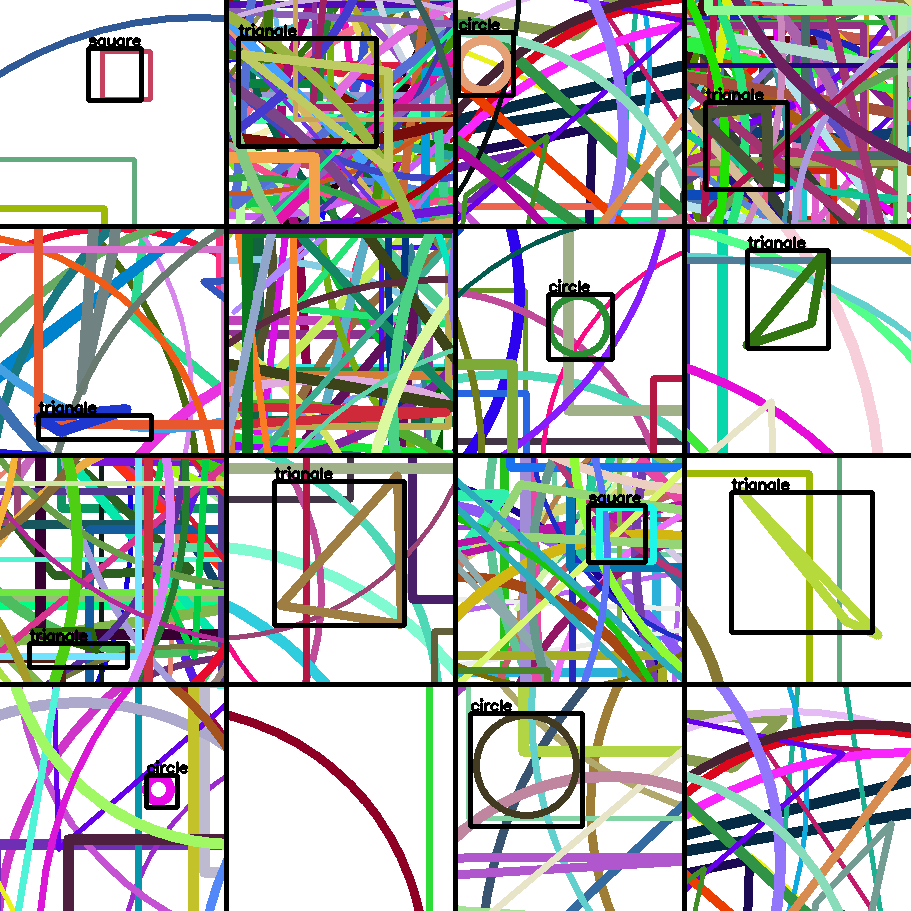
\includegraphics[width=\textwidth]{img/simple_detection.png}
%     \caption{Detections by simple model 1 7x7 feature map to 4 coordinates and fully connected for class}
%     \label{fig:my_label}
% \end{figure}

\subsubsection{Full SSD, convolution and multiple feature layers}
Training SSD clear vs pretrained
batch size 256, batches per epoch 500
% \begin{table}[]
% \begin{tabular}{llll}
%  Epochs &  random mAP & pretrained mAP & imgNet pret. mAP \\
%  1 & 0.11 & 0.76 & 0.53 \\
%  &   & &\\
%  &  & &
% \end{tabular}
% \caption{bla bla}
%     \label{tab:Comparison of training}
% \end{table}



\subsection{Applying SSD trained on artificial dataset to realistic images}

\subsection{Measuring the impact of number of classes}

\section{Speeding up video procesing}

\chapter*{Conclusion}
\addcontentsline{toc}{chapter}{Conclusion}


\subsection*{Future work}



%%% Bibliography
%%% Bibliography (literature used as a source)
%%%
%%% We employ bibTeX to construct the bibliography. It processes
%%% citations in the text (e.g., the \cite{...} macro) and looks up
%%% relevant entries in the bibliography.bib file.
%%%
%%% The \bibliographystyle command selects, which style will be used
%%% for references from the text. The argument in curly brackets is
%%% the name of the corresponding style file (*.bst). Both styles
%%% mentioned in this template are included in LaTeX distributions.

%\bibliographystyle{plain}    %% Author (year)
%\bibliographystyle{unsrt}     %% [number]

\renewcommand{\bibname}{Bibliography}

%%% Generate the bibliography. Beware that if you cited no works,
%%% the empty list will be omitted completely.

\bibliography{bibliography}

%%% If case you prefer to write the bibliography manually (without bibTeX),
%%% you can use the following. Please follow the ISO 690 standard and
%%% citation conventions of your field of research.

% \begin{thebibliography}{99}
%
% \bibitem{lamport94}
%   {\sc Lamport,} Leslie.
%   \emph{\LaTeX: A Document Preparation System}.
%   2nd edition.
%   Massachusetts: Addison Wesley, 1994.
%   ISBN 0-201-52983-1.
%
% \end{thebibliography}


\appendix
\chapter{Implementation of SSD}

\chapter{Some other implementation appendix}




%%% Figures used in the thesis (consider if this is needed)
%\listoffigures
% list of figures je dobrej do knizek co maj 500+ stranek, tady to je uplna zbytecnost.

%%% Tables used in the thesis (consider if this is needed)
%%% In mathematical theses, it could be better to move the list of tables to the beginning of the thesis.
%%%\listoftables

%%% Abbreviations used in the thesis, if any, including their explanation
%%% In mathematical theses, it could be better to move the list of abbreviations to the beginning of the thesis.
%%%\chapwithtoc{List of Abbreviations}

%%% Attachments to the bachelor thesis, if any. Each attachment must be
%%% referred to at least once from the text of the thesis. Attachments
%%% are numbered.
%%%
%%% The printed version should preferably contain attachments, which can be
%%% read (additional tables and charts, supplementary text, examples of
%%% program output, etc.). The electronic version is more suited for attachments
%%% which will likely be used in an electronic form rather than read (program
%%% source code, data files, interactive charts, etc.). Electronic attachments
%%% should be uploaded to SIS and optionally also included in the thesis on a~CD/DVD.
%%% Allowed file formats are specified in provision of the rector no. 23/2016.
%\chapwithtoc{Attachments}

\openright
\end{document}
